\documentclass[tikz]{standalone}
\usetikzlibrary{positioning}

\begin{document}
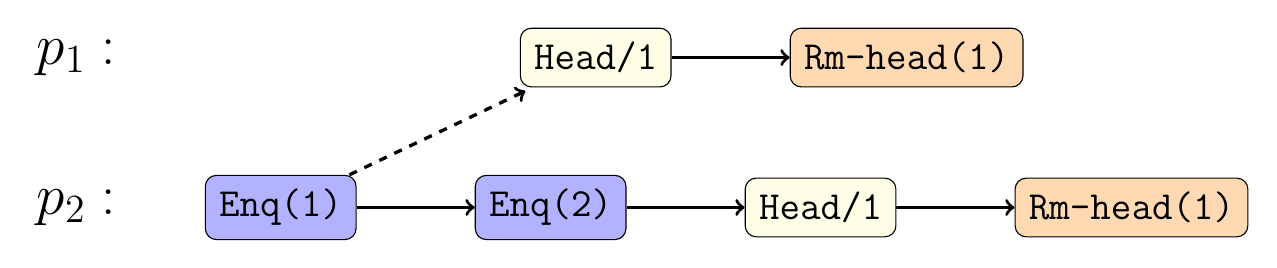
\begin{tikzpicture}
\tikzset{
  enq-op/.style = {rectangle, rounded corners, fill = blue!30, draw, font = \Large, inner sep = 5pt},
  deq-hd/.style = {rectangle, rounded corners, fill = yellow!10, draw, font = \Large, inner sep = 5pt},
  deq-rh/.style = {rectangle, rounded corners, fill = orange!30, draw, font = \Large, inner sep = 5pt},
  process/.style = {font = \huge},
  po/.style = {->, very thick},
  vis/.style = {->, shorten >= 3pt, very thick, dashed}
}

  \node (p1) [process] {$p_1:$};
  \node (p1-deq1-hd) [deq-hd, right = 5.0cm of p1] {\texttt{Head/1}};
  \node (p1-deq1-rh) [deq-rh, right = 1.5cm of p1-deq1-hd] {\texttt{Rm-head(1)}};

  \node (p2) [process, below = 1.2cm of p1] {$p_2:$};
  \node (p2-enq1) [enq-op, right = 1.0cm of p2] {\texttt{Enq(1)}};
  \node (p2-enq2) [enq-op, right = 1.5cm of p2-enq1] {\texttt{Enq(2)}};
  \node (p2-deq1-hd) [deq-hd, right = 1.5cm of p2-enq2] {\texttt{Head/1}};
  \node (p2-deq1-rh) [deq-rh, right = 1.5cm of p2-deq1-hd] {\texttt{Rm-head(1)}};

  \draw [po] (p1-deq1-hd) to (p1-deq1-rh);
  \draw [po] (p2-enq1) to (p2-enq2);
  \draw [po] (p2-enq2) to (p2-deq1-hd);
  \draw [po] (p2-deq1-hd) to (p2-deq1-rh);

  \draw [vis] (p2-enq1) to (p1-deq1-hd);
  %\draw [vis] (p1-deq1-rh) to (p2-deq1-hd);
\end{tikzpicture}
\end{document}